\SourceLeaf{312}

\Needspace{8\baselineskip}\textls{Die zweite Auflösungsart.}

Es seien $\xi$, $\eta$ [die] Coordinaten des Mittelpunkts des durch die drei Punkte gelegten Kreises, $\rho$ dessen Halbmesser. Man mache, wie vorhin

\[
a'' - a' = h\cos A, \qquad a - a'' = h'\cos A', \qquad a' - a = h''\cos A'',
\]
\[
b'' - b' = h\sin A, \qquad b - b'' = h'\sin A', \qquad b' - b = h''\sin A''.
\]

Man hat dann

\[
\begin{aligned}
\xi &= a + \rho\sin(A'+A''-A)\\ &= a' + \rho\sin(A''+A-A')\\ &= a'' + \rho\sin(A+A'-A''),
\end{aligned}
\]
\[
\begin{aligned}
\eta &= b - \rho\cos(A'+A''-A)\\ &= b' - \rho\cos(A''+A-A')\\ &= b'' - \rho\cos(A+A'-A''),
\end{aligned}
\]
\[
\rho = \dfrac{h}{\sin(A''-A')} = \dfrac{h'}{\sin(A-A'')} = \dfrac{h''}{\sin(A'-A)}.
\]

\begin{center}\resizebox{5.3cm}{!}{%
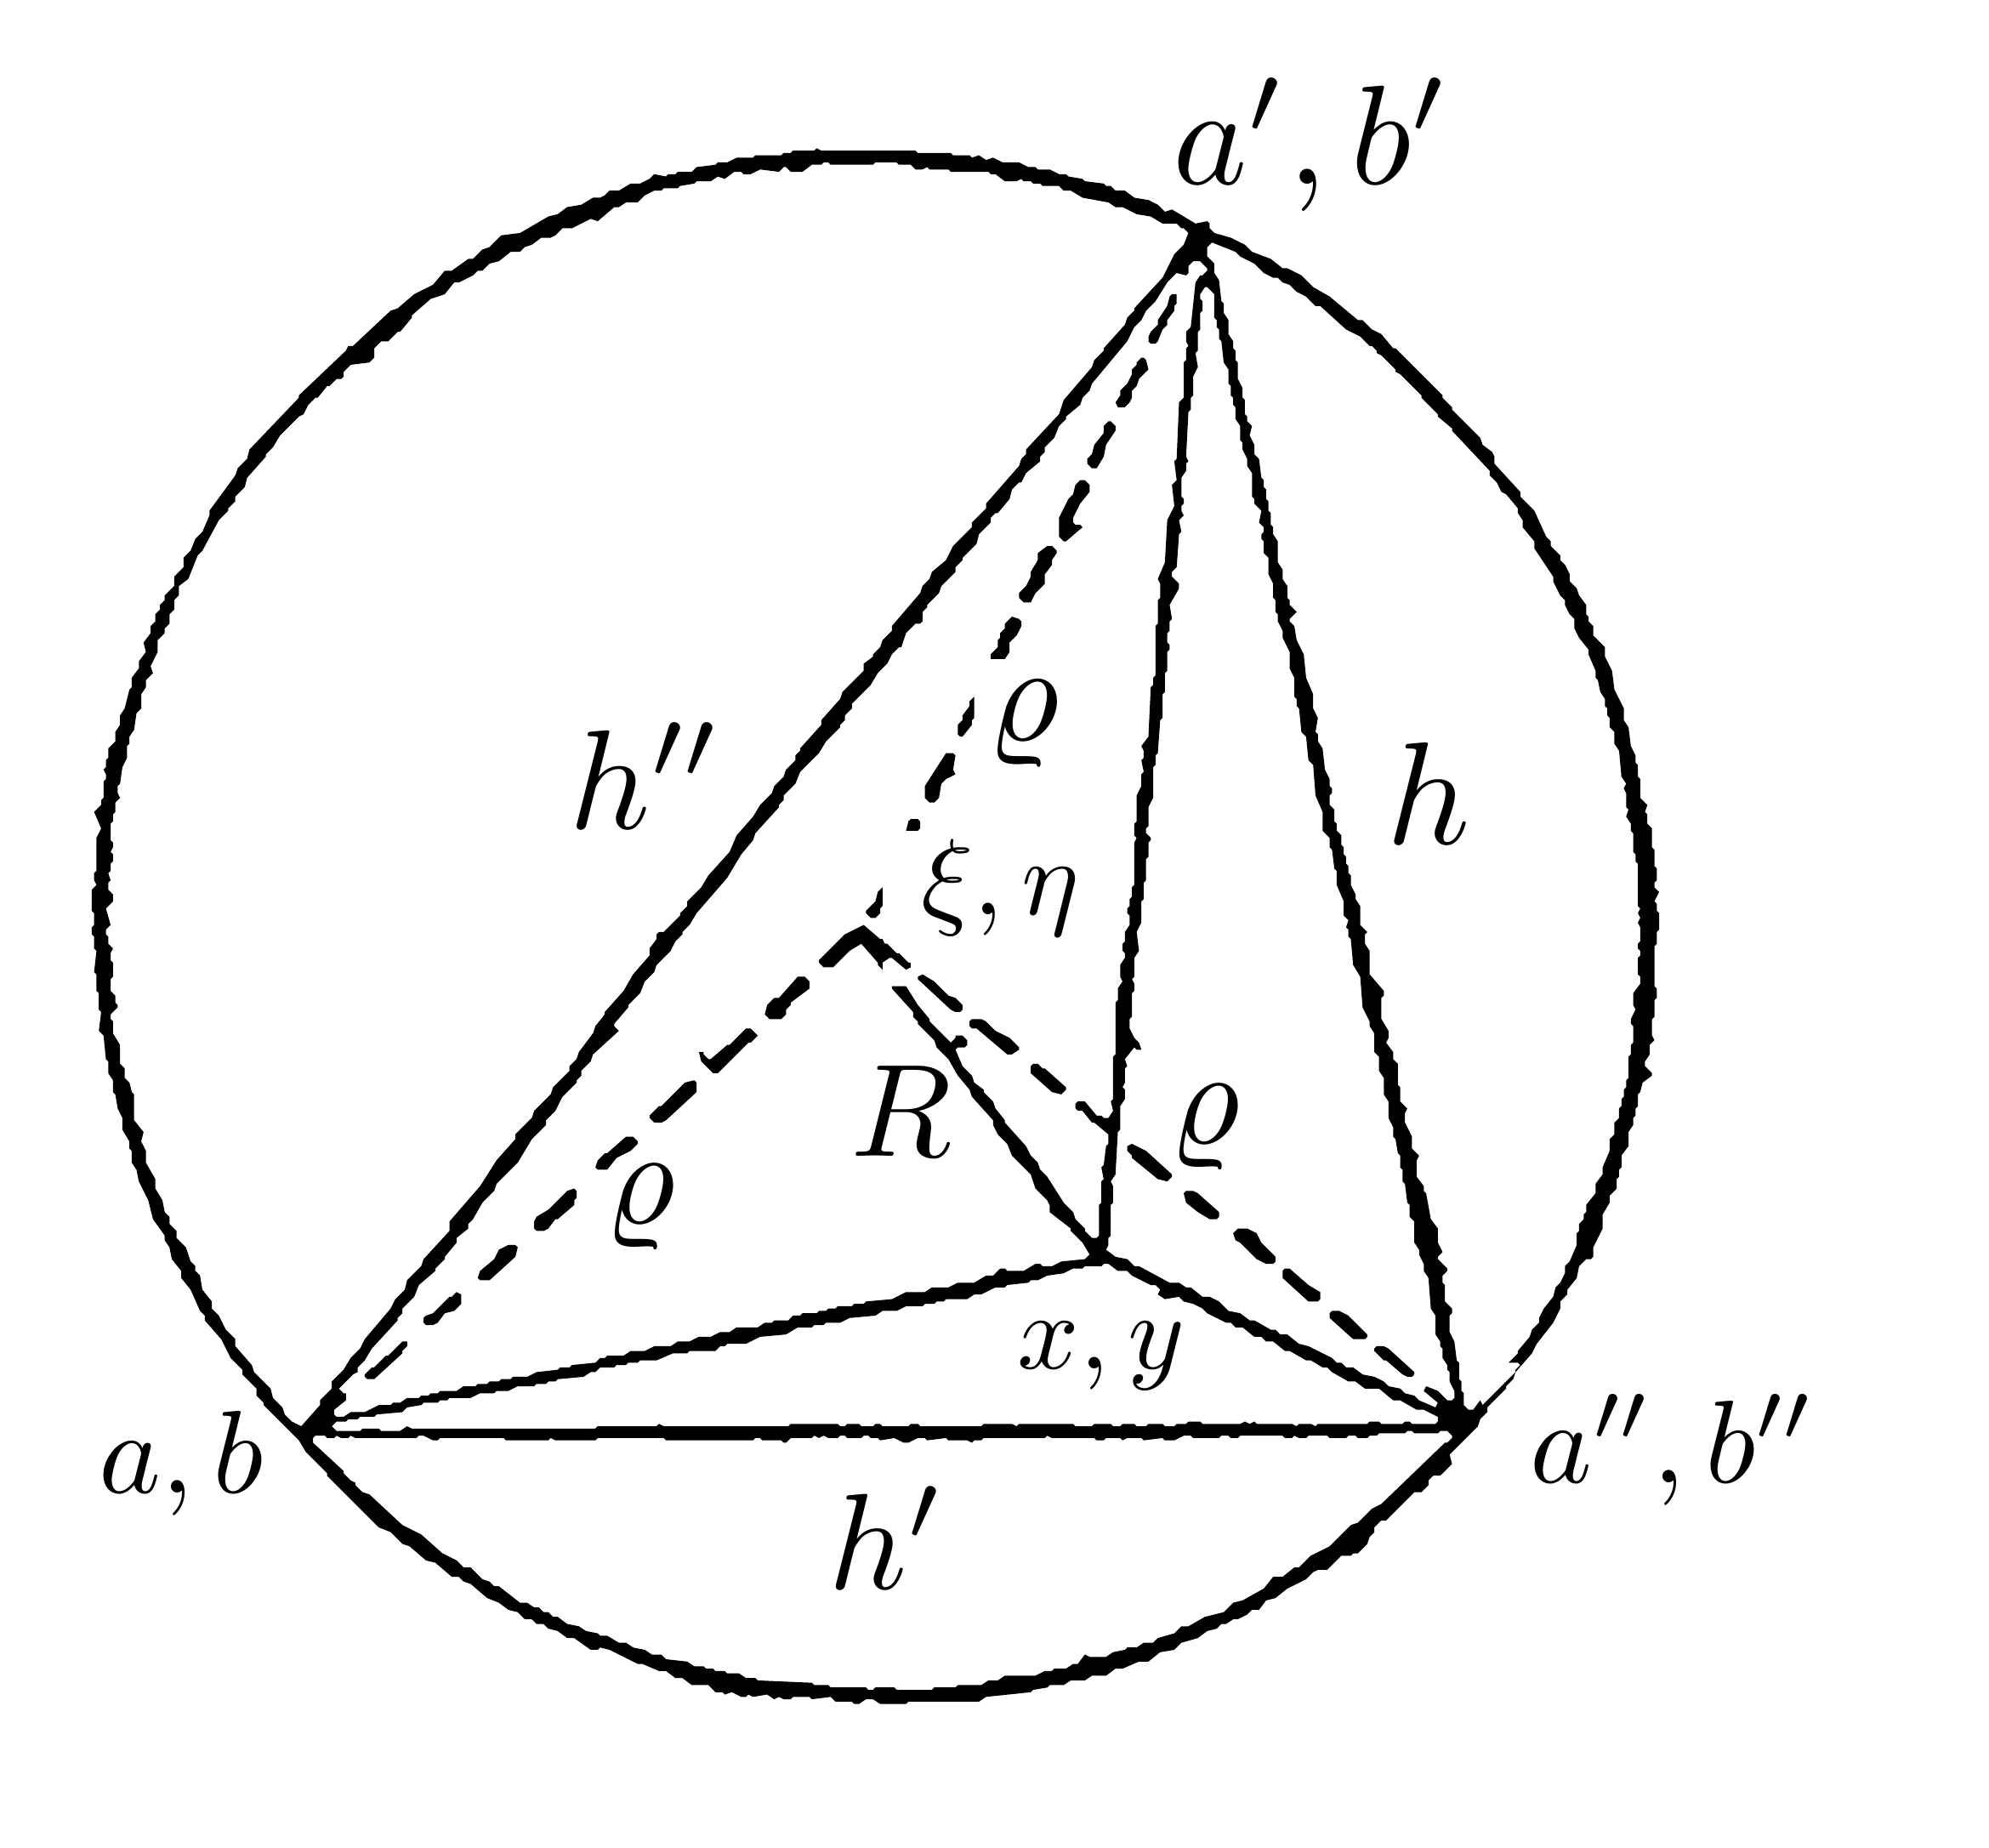
\begin{tikzpicture}[x=1pt,y=-1pt]
\path[use as bounding box] (0,0) rectangle (825,765);
\path[fill=black,draw=none,even odd rule]
(303,57) -- (299,59) -- (295,59) -- (294,60) -- (286,61) -- (284,63) -- (278,63) -- (277,64) -- (274,64) -- (273,65) -- (268,64) -- (266,66) -- (262,68) -- (258,68) -- (253,71) -- (249,71) -- (247,73) -- (245,74) -- (242,74) -- (237,77) -- (231,78) -- (227,81) -- (223,82) -- (211,89) -- (203,90) -- (198,95) -- (195,96) -- (191,100) -- (189,100) -- (182,105) -- (179,105) -- (174,111) -- (166,115) -- (159,121) -- (156,122) -- (140,137) -- (138,137) -- (137,139) -- (117,158) -- (117,159) -- (96,181) -- (95,185) -- (91,189) -- (90,192) -- (79,207) -- (79,209) -- (76,216) -- (73,219) -- (71,224) -- (68,227) -- (68,231) -- (64,235) -- (64,239) -- (60,243) -- (60,245) -- (58,247) -- (58,249) -- (56,251) -- (56,254) -- (54,256) -- (54,259) -- (51,263) -- (52,267) -- (49,271) -- (49,274) -- (46,278) -- (46,282) -- (45,283) -- (43,291) -- (41,294) -- (41,298) -- (39,301) -- (39,305) -- (36,308) -- (36,312) -- (35,313) -- (35,316) -- (34,317) -- (35,319) -- (35,321) -- (34,322) -- (34,329) -- (33,330) -- (33,332) -- (30,335) -- (33,342) -- (31,346) -- (31,360) -- (30,361) -- (30,364) -- (31,366) -- (29,368) -- (29,377) -- (30,378) -- (30,383) -- (29,384) -- (29,387) -- (30,388) -- (30,393) -- (31,394) -- (30,403) -- (31,404) -- (31,411) -- (32,412) -- (32,419) -- (33,420) -- (32,428) -- (34,430) -- (35,440) -- (36,441) -- (36,446) -- (38,449) -- (38,454) -- (39,455) -- (40,461) -- (42,465) -- (42,470) -- (45,475) -- (45,478) -- (46,479) -- (46,484) -- (48,487) -- (49,492) -- (53,500) -- (55,508) -- (60,515) -- (60,517) -- (62,520) -- (63,525) -- (67,530) -- (67,533) -- (71,538) -- (75,547) -- (77,549) -- (77,551) -- (84,559) -- (88,567) -- (93,572) -- (93,574) -- (99,580) -- (99,583) -- (102,586) -- (102,587) -- (117,602) -- (120,607) -- (129,616) -- (129,617) -- (151,639) -- (156,641) -- (161,646) -- (164,647) -- (171,653) -- (175,654) -- (182,660) -- (185,660) -- (187,662) -- (190,663) -- (197,669) -- (202,671) -- (206,674) -- (210,675) -- (213,678) -- (216,678) -- (218,680) -- (221,680) -- (223,682) -- (227,683) -- (231,686) -- (234,686) -- (241,691) -- (244,691) -- (245,690) -- (249,691) -- (261,697) -- (263,697) -- (270,700) -- (273,700) -- (277,703) -- (280,703) -- (284,706) -- (291,706) -- (294,709) -- (297,709) -- (298,710) -- (301,709) -- (305,711) -- (307,711) -- (308,710) -- (310,711) -- (316,710) -- (319,712) -- (321,711) -- (323,712) -- (326,712) -- (327,711) -- (334,711) -- (335,712) -- (343,711) -- (345,713) -- (352,713) -- (353,714) -- (355,714) -- (358,712) -- (361,712) -- (364,714) -- (375,714) -- (376,713) -- (406,713) -- (409,711) -- (428,709) -- (429,708) -- (435,707) -- (436,706) -- (442,706) -- (445,704) -- (451,704) -- (454,702) -- (460,702) -- (464,699) -- (467,699) -- (474,696) -- (478,696) -- (483,692) -- (489,691) -- (492,688) -- (499,686) -- (503,683) -- (507,682) -- (509,680) -- (511,680) -- (514,678) -- (516,678) -- (520,676) -- (522,674) -- (525,674) -- (528,670) -- (532,669) -- (537,665) -- (545,661) -- (548,658) -- (550,657) -- (554,657) -- (560,651) -- (564,651) -- (565,650) -- (567,650) -- (571,646) -- (572,643) -- (574,641) -- (574,639) -- (577,636) -- (579,636) -- (591,624) -- (594,624) -- (597,621) -- (597,619) -- (599,617) -- (602,617) -- (607,612) -- (606,608) -- (618,596) -- (619,593) -- (622,590) -- (622,588) -- (630,580) -- (630,579) -- (633,576) -- (634,573) -- (641,565) -- (643,561) -- (650,552) -- (653,546) -- (653,543) -- (656,540) -- (656,538) -- (660,533) -- (661,528) -- (664,525) -- (666,525) -- (667,524) -- (667,520) -- (671,512) -- (671,506) -- (674,501) -- (674,498) -- (677,495) -- (677,491) -- (678,490) -- (678,487) -- (679,486) -- (679,481) -- (682,477) -- (682,471) -- (684,468) -- (684,465) -- (685,464) -- (685,461) -- (686,460) -- (686,455) -- (687,454) -- (688,450) -- (692,447) -- (692,446) -- (689,443) -- (689,441) -- (691,438) -- (691,434) -- (693,432) -- (692,430) -- (692,423) -- (693,422) -- (693,415) -- (694,414) -- (694,410) -- (693,409) -- (693,392) -- (694,391) -- (694,386) -- (695,385) -- (695,378) -- (694,377) -- (694,374) -- (693,373) -- (695,369) -- (693,367) -- (693,365) -- (694,364) -- (694,359) -- (693,358) -- (693,351) -- (692,350) -- (692,342) -- (690,340) -- (690,336) -- (689,335) -- (690,332) -- (687,329) -- (687,321) -- (686,320) -- (686,315) -- (685,314) -- (685,311) -- (683,307) -- (682,299) -- (680,296) -- (680,291) -- (676,283) -- (675,275) -- (672,269) -- (672,265) -- (667,260) -- (667,256) -- (665,254) -- (665,252) -- (664,251) -- (664,247) -- (661,243) -- (660,240) -- (657,237) -- (657,234) -- (655,230) -- (653,228) -- (653,226) -- (649,222) -- (649,220) -- (647,218) -- (642,207) -- (636,201) -- (636,199) -- (625,187) -- (625,184) -- (624,182) -- (620,179) -- (619,176) -- (607,164) -- (607,163) -- (603,159) -- (603,158) -- (583,138) -- (582,138) -- (577,132) -- (573,130) -- (569,126) -- (567,126) -- (555,116) -- (548,112) -- (543,107) -- (537,104) -- (535,104) -- (530,100) -- (522,97) -- (519,94) -- (513,91) -- (506,89) -- (504,87) -- (504,85) -- (503,84) -- (498,85) -- (488,79) -- (485,80) -- (482,77) -- (478,75) -- (472,74) -- (468,71) -- (464,71) -- (462,69) -- (460,69) -- (459,68) -- (451,67) -- (450,66) -- (444,65) -- (443,64) -- (440,64) -- (436,62) -- (431,62) -- (430,61) -- (427,61) -- (423,59) -- (416,59) -- (412,57) -- (409,58) -- (406,56) -- (403,57) -- (402,56) -- (395,56) -- (394,55) -- (380,55) -- (379,54) -- (339,54) -- (337,53) -- (336,54) -- (327,54) -- (326,55) -- (323,55) -- (322,56) -- (311,56) -- (310,57) -- cycle
(607,600) -- (607,601) -- (605,603) -- (604,603) -- (577,629) -- (573,631) -- (567,637) -- (564,638) -- (555,647) -- (547,651) -- (542,656) -- (540,656) -- (535,660) -- (531,660) -- (527,665) -- (518,670) -- (514,671) -- (510,675) -- (502,677) -- (495,681) -- (492,681) -- (489,684) -- (482,686) -- (480,688) -- (476,688) -- (473,690) -- (469,690) -- (468,691) -- (463,692) -- (460,694) -- (453,694) -- (451,693) -- (448,697) -- (446,697) -- (443,699) -- (438,699) -- (437,700) -- (434,700) -- (430,702) -- (417,702) -- (414,704) -- (410,704) -- (407,706) -- (397,706) -- (396,707) -- (387,707) -- (386,708) -- (371,708) -- (370,707) -- (362,707) -- (361,708) -- (359,708) -- (358,707) -- (343,707) -- (342,706) -- (336,706) -- (335,705) -- (312,704) -- (311,703) -- (307,703) -- (304,701) -- (299,701) -- (298,700) -- (294,700) -- (293,699) -- (290,699) -- (289,698) -- (285,698) -- (282,696) -- (273,695) -- (271,693) -- (267,693) -- (264,691) -- (259,690) -- (256,688) -- (253,688) -- (248,685) -- (245,685) -- (244,684) -- (239,683) -- (236,681) -- (231,680) -- (227,677) -- (225,677) -- (223,675) -- (221,675) -- (219,673) -- (217,673) -- (214,671) -- (211,671) -- (202,664) -- (200,664) -- (198,662) -- (195,661) -- (190,656) -- (187,656) -- (184,653) -- (178,650) -- (169,642) -- (161,638) -- (147,625) -- (144,624) -- (141,621) -- (141,620) -- (139,619) -- (136,616) -- (136,615) -- (123,603) -- (123,601) -- (124,600) -- (128,600) -- (129,601) -- (132,601) -- (133,600) -- (135,601) -- (138,601) -- (139,600) -- (141,601) -- (167,601) -- (168,600) -- (170,600) -- (174,602) -- (176,602) -- (177,601) -- (204,601) -- (205,602) -- (223,602) -- (224,601) -- (226,602) -- (243,602) -- (244,601) -- (272,601) -- (273,602) -- (310,602) -- (311,601) -- (313,601) -- (314,602) -- (322,602) -- (323,603) -- (324,603) -- (326,601) -- (335,601) -- (336,600) -- (338,601) -- (340,600) -- (342,601) -- (346,601) -- (347,600) -- (349,600) -- (350,601) -- (356,601) -- (357,600) -- (359,600) -- (360,601) -- (363,601) -- (364,602) -- (370,601) -- (374,603) -- (376,603) -- (380,601) -- (383,601) -- (384,602) -- (392,601) -- (393,602) -- (401,602) -- (403,603) -- (404,602) -- (407,602) -- (408,601) -- (434,601) -- (435,600) -- (437,601) -- (455,601) -- (456,602) -- (459,602) -- (460,601) -- (466,601) -- (467,602) -- (469,601) -- (475,601) -- (476,602) -- (484,601) -- (485,602) -- (489,602) -- (493,600) -- (496,600) -- (497,601) -- (508,601) -- (509,600) -- (512,600) -- (513,601) -- (516,601) -- (517,600) -- (535,600) -- (536,601) -- (539,601) -- (540,600) -- (542,601) -- (545,601) -- (546,600) -- (554,600) -- (555,601) -- (562,601) -- (563,600) -- (566,600) -- (567,601) -- (571,601) -- (572,600) -- (575,600) -- (576,599) -- (587,599) -- (588,598) -- (590,598) -- (591,599) -- (601,599) -- (602,598) -- (605,598) -- cycle
(601,592) -- (601,594) -- (600,595) -- (590,595) -- (589,594) -- (587,594) -- (586,595) -- (577,595) -- (576,594) -- (572,594) -- (571,595) -- (550,595) -- (549,596) -- (547,595) -- (542,595) -- (541,596) -- (539,595) -- (524,595) -- (523,594) -- (521,595) -- (519,594) -- (517,595) -- (501,595) -- (500,594) -- (495,594) -- (494,595) -- (490,595) -- (489,596) -- (485,596) -- (484,595) -- (478,595) -- (477,596) -- (473,596) -- (472,595) -- (467,595) -- (466,596) -- (463,596) -- (462,595) -- (455,595) -- (454,596) -- (447,596) -- (446,595) -- (423,595) -- (422,596) -- (420,595) -- (408,595) -- (407,596) -- (381,596) -- (380,595) -- (377,595) -- (376,596) -- (365,596) -- (364,595) -- (362,595) -- (361,596) -- (356,596) -- (355,595) -- (350,595) -- (349,596) -- (347,596) -- (346,595) -- (326,595) -- (325,596) -- (272,596) -- (270,595) -- (269,596) -- (244,596) -- (243,597) -- (165,597) -- (163,596) -- (160,598) -- (152,598) -- (151,597) -- (144,597) -- (143,598) -- (133,598) -- (131,596) -- (133,594) -- (137,594) -- (138,593) -- (142,593) -- (143,592) -- (149,592) -- (150,591) -- (161,590) -- (163,588) -- (169,587) -- (170,586) -- (176,586) -- (177,585) -- (180,585) -- (181,584) -- (190,584) -- (194,582) -- (200,582) -- (201,581) -- (206,581) -- (210,579) -- (217,579) -- (218,578) -- (222,578) -- (223,577) -- (226,577) -- (227,576) -- (238,575) -- (241,573) -- (243,573) -- (245,571) -- (251,571) -- (252,570) -- (256,570) -- (257,569) -- (261,569) -- (262,568) -- (269,568) -- (276,565) -- (282,565) -- (283,564) -- (294,564) -- (296,562) -- (298,562) -- (299,561) -- (307,561) -- (313,558) -- (324,557) -- (329,554) -- (335,554) -- (336,553) -- (340,553) -- (341,552) -- (347,552) -- (351,550) -- (362,549) -- (365,547) -- (371,547) -- (375,545) -- (382,545) -- (383,544) -- (387,544) -- (388,543) -- (391,543) -- (392,542) -- (401,542) -- (404,540) -- (407,540) -- (413,537) -- (417,537) -- (418,536) -- (427,535) -- (428,534) -- (431,534) -- (435,532) -- (442,531) -- (446,529) -- (450,529) -- (451,528) -- (458,528) -- (459,527) -- (461,527) -- (465,530) -- (469,530) -- (471,532) -- (479,536) -- (481,536) -- (483,538) -- (482,540) -- (485,542) -- (491,541) -- (493,543) -- (497,544) -- (501,546) -- (503,548) -- (511,552) -- (513,552) -- (515,554) -- (518,554) -- (523,558) -- (526,558) -- (528,560) -- (531,560) -- (536,564) -- (538,564) -- (545,568) -- (547,568) -- (552,571) -- (554,571) -- (556,573) -- (563,577) -- (566,577) -- (570,580) -- (576,580) -- (582,585) -- (585,585) -- (592,589) -- (595,589) -- cycle
(502,112) -- (503,112) -- (506,115) -- (506,125) -- (507,126) -- (507,129) -- (508,130) -- (508,134) -- (509,135) -- (510,144) -- (512,147) -- (512,153) -- (513,154) -- (513,158) -- (514,159) -- (514,162) -- (515,163) -- (515,168) -- (517,171) -- (517,177) -- (518,178) -- (518,181) -- (520,185) -- (520,188) -- (522,191) -- (522,201) -- (523,202) -- (523,204) -- (526,207) -- (525,212) -- (527,214) -- (527,216) -- (526,217) -- (526,219) -- (527,220) -- (527,225) -- (529,227) -- (529,234) -- (531,238) -- (531,244) -- (532,245) -- (532,250) -- (533,251) -- (533,254) -- (535,258) -- (535,261) -- (538,267) -- (538,274) -- (540,278) -- (540,286) -- (541,287) -- (541,290) -- (542,291) -- (543,301) -- (545,303) -- (546,313) -- (548,315) -- (549,328) -- (552,335) -- (552,343) -- (555,346) -- (555,350) -- (556,351) -- (557,359) -- (558,360) -- (558,366) -- (561,373) -- (561,379) -- (563,381) -- (562,384) -- (563,385) -- (563,388) -- (564,389) -- (565,400) -- (568,405) -- (569,418) -- (572,424) -- (572,426) -- (574,429) -- (574,437) -- (576,439) -- (576,445) -- (578,448) -- (578,455) -- (580,458) -- (580,465) -- (582,469) -- (582,473) -- (583,474) -- (584,480) -- (585,481) -- (585,486) -- (586,487) -- (586,492) -- (587,493) -- (588,501) -- (589,502) -- (589,507) -- (591,509) -- (591,518) -- (593,521) -- (593,523) -- (595,527) -- (595,530) -- (597,533) -- (598,546) -- (600,549) -- (600,557) -- (602,560) -- (602,562) -- (603,563) -- (603,567) -- (605,570) -- (605,572) -- (606,573) -- (606,577) -- (608,581) -- (608,584) -- (607,585) -- (605,585) -- (601,581) -- (596,579) -- (595,581) -- (601,586) -- (600,588) -- (593,585) -- (591,583) -- (587,582) -- (585,580) -- (580,579) -- (578,577) -- (574,575) -- (569,574) -- (565,571) -- (562,571) -- (560,569) -- (558,569) -- (556,567) -- (546,562) -- (542,561) -- (537,557) -- (534,557) -- (532,555) -- (530,555) -- (523,551) -- (521,551) -- (517,548) -- (512,547) -- (508,543) -- (504,541) -- (501,541) -- (496,537) -- (494,537) -- (491,535) -- (487,535) -- (474,528) -- (472,528) -- (469,525) -- (464,524) -- (460,521) -- (461,519) -- (461,516) -- (462,515) -- (462,502) -- (463,501) -- (463,494) -- (462,492) -- (464,489) -- (465,471) -- (466,470) -- (466,460) -- (468,457) -- (468,453) -- (467,452) -- (468,450) -- (468,444) -- (469,443) -- (468,440) -- (472,435) -- (473,436) -- (475,436) -- (474,433) -- (472,431) -- (470,427) -- (470,423) -- (471,422) -- (471,412) -- (472,411) -- (472,408) -- (471,406) -- (472,405) -- (472,397) -- (474,394) -- (473,386) -- (475,382) -- (475,373) -- (476,372) -- (476,365) -- (477,364) -- (477,355) -- (478,354) -- (478,348) -- (479,347) -- (479,346) -- (477,344) -- (477,342) -- (478,341) -- (478,333) -- (480,329) -- (480,316) -- (481,315) -- (481,311) -- (482,310) -- (483,296) -- (484,295) -- (484,285) -- (485,284) -- (485,276) -- (486,275) -- (486,267) -- (487,266) -- (487,264) -- (486,263) -- (486,259) -- (487,258) -- (487,254) -- (488,253) -- (487,247) -- (491,240) -- (491,238) -- (488,235) -- (488,233) -- (490,231) -- (491,217) -- (492,216) -- (491,211) -- (493,209) -- (492,207) -- (492,205) -- (493,204) -- (493,202) -- (492,201) -- (492,193) -- (494,190) -- (494,187) -- (495,186) -- (494,184) -- (495,165) -- (496,164) -- (496,159) -- (497,158) -- (497,150) -- (499,146) -- (498,140) -- (499,139) -- (499,131) -- (500,130) -- (500,123) -- (501,122) -- (501,118) -- (500,117) -- (500,115) -- cycle
(574,563) -- (574,564) -- (578,568) -- (579,568) -- (586,574) -- (588,575) -- (590,575) -- (591,574) -- (591,573) -- (580,563) -- (578,562) -- (575,562) -- cycle
(555,548) -- (555,550) -- (565,559) -- (570,559) -- (571,558) -- (571,557) -- (563,549) -- (559,547) -- (556,547) -- cycle
(535,530) -- (535,533) -- (546,543) -- (550,543) -- (551,542) -- (551,539) -- (546,536) -- (538,529) -- (536,529) -- cycle
(514,514) -- (515,517) -- (517,518) -- (524,525) -- (528,527) -- (531,527) -- (532,526) -- (532,524) -- (526,518) -- (524,514) -- (520,512) -- (516,512) -- cycle
(493,497) -- (494,501) -- (499,505) -- (504,508) -- (507,508) -- (508,507) -- (508,505) -- (499,497) -- (497,496) -- (494,496) -- cycle
(469,477) -- (469,479) -- (471,481) -- (471,482) -- (482,491) -- (486,492) -- (488,490) -- (488,489) -- (477,479) -- (471,476) -- cycle
(500,101) -- (503,104) -- (503,105) -- (501,107) -- (500,107) -- (498,110) -- (496,129) -- (494,131) -- (494,135) -- (495,137) -- (494,138) -- (494,143) -- (493,144) -- (493,159) -- (491,161) -- (490,185) -- (489,186) -- (490,194) -- (488,196) -- (489,205) -- (486,211) -- (485,229) -- (482,236) -- (483,238) -- (483,244) -- (482,245) -- (482,255) -- (481,256) -- (481,277) -- (480,278) -- (480,281) -- (479,282) -- (478,303) -- (475,307) -- (476,309) -- (476,312) -- (475,313) -- (476,318) -- (475,319) -- (475,324) -- (473,328) -- (473,339) -- (472,340) -- (472,345) -- (473,346) -- (472,348) -- (472,366) -- (471,367) -- (471,371) -- (470,372) -- (470,375) -- (469,376) -- (469,378) -- (470,379) -- (470,383) -- (468,386) -- (468,390) -- (467,391) -- (467,394) -- (468,395) -- (468,397) -- (466,400) -- (466,405) -- (467,407) -- (465,410) -- (465,415) -- (464,416) -- (464,438) -- (463,439) -- (463,457) -- (462,458) -- (463,462) -- (461,465) -- (459,465) -- (458,464) -- (456,464) -- (451,458) -- (448,458) -- (447,459) -- (447,461) -- (448,462) -- (450,462) -- (454,467) -- (455,467) -- (461,472) -- (461,476) -- (460,477) -- (459,485) -- (458,486) -- (459,491) -- (458,492) -- (458,501) -- (457,502) -- (457,515) -- (456,516) -- (454,516) -- (451,513) -- (451,512) -- (447,508) -- (446,505) -- (442,501) -- (435,490) -- (432,487) -- (431,484) -- (428,481) -- (426,477) -- (417,467) -- (417,466) -- (413,461) -- (412,458) -- (408,454) -- (408,453) -- (404,450) -- (403,447) -- (399,443) -- (396,436) -- (397,435) -- (400,435) -- (401,434) -- (401,432) -- (399,430) -- (396,430) -- (396,431) -- (394,433) -- (385,424) -- (385,423) -- (380,417) -- (375,409) -- (369,409) -- (369,410) -- (378,420) -- (378,422) -- (380,424) -- (380,425) -- (387,432) -- (388,435) -- (393,440) -- (397,447) -- (402,453) -- (403,456) -- (412,466) -- (412,468) -- (414,472) -- (418,476) -- (420,481) -- (428,489) -- (430,495) -- (435,500) -- (436,502) -- (436,505) -- (445,512) -- (445,513) -- (450,518) -- (453,523) -- (451,525) -- (441,526) -- (437,528) -- (433,528) -- (432,527) -- (430,527) -- (425,530) -- (418,530) -- (417,529) -- (415,529) -- (412,532) -- (409,532) -- (404,535) -- (397,535) -- (393,537) -- (386,537) -- (383,539) -- (375,539) -- (369,542) -- (358,543) -- (357,544) -- (353,544) -- (352,545) -- (346,545) -- (345,546) -- (342,546) -- (341,547) -- (338,547) -- (337,548) -- (331,548) -- (330,549) -- (327,549) -- (325,551) -- (319,551) -- (318,552) -- (315,552) -- (312,554) -- (303,554) -- (300,556) -- (296,556) -- (292,558) -- (287,558) -- (283,560) -- (278,560) -- (275,562) -- (268,562) -- (264,564) -- (258,564) -- (255,566) -- (248,566) -- (247,567) -- (245,567) -- (243,569) -- (233,570) -- (232,571) -- (228,571) -- (227,572) -- (218,573) -- (214,575) -- (208,575) -- (207,576) -- (203,576) -- (202,577) -- (198,577) -- (197,578) -- (193,578) -- (192,579) -- (187,579) -- (184,581) -- (177,581) -- (176,582) -- (173,582) -- (172,583) -- (169,583) -- (168,584) -- (163,584) -- (160,586) -- (157,586) -- (156,587) -- (151,587) -- (145,590) -- (139,590) -- (136,592) -- (133,592) -- (132,591) -- (132,589) -- (137,585) -- (137,582) -- (136,582) -- (134,580) -- (140,574) -- (142,573) -- (142,571) -- (145,568) -- (148,563) -- (159,551) -- (159,550) -- (161,548) -- (161,546) -- (166,541) -- (168,536) -- (175,530) -- (175,529) -- (179,525) -- (179,524) -- (184,518) -- (184,516) -- (189,512) -- (189,510) -- (191,508) -- (195,501) -- (200,496) -- (201,493) -- (210,484) -- (216,474) -- (222,468) -- (222,466) -- (226,462) -- (229,456) -- (235,450) -- (235,449) -- (237,447) -- (237,445) -- (241,441) -- (242,438) -- (253,428) -- (251,426) -- (251,425) -- (257,418) -- (257,417) -- (262,412) -- (264,407) -- (268,403) -- (269,400) -- (275,394) -- (277,390) -- (280,387) -- (280,386) -- (283,383) -- (286,378) -- (299,363) -- (305,353) -- (310,347) -- (311,344) -- (321,333) -- (321,332) -- (323,330) -- (323,328) -- (328,323) -- (330,318) -- (338,310) -- (341,305) -- (347,299) -- (347,298) -- (349,296) -- (349,294) -- (352,291) -- (352,289) -- (360,281) -- (363,276) -- (367,272) -- (369,268) -- (372,265) -- (373,265) -- (375,259) -- (379,255) -- (381,255) -- (382,254) -- (382,250) -- (384,248) -- (384,247) -- (389,242) -- (390,239) -- (396,233) -- (396,231) -- (399,228) -- (399,227) -- (405,221) -- (406,217) -- (411,212) -- (411,210) -- (413,208) -- (414,208) -- (419,202) -- (420,198) -- (423,195) -- (424,195) -- (426,191) -- (432,186) -- (432,184) -- (434,182) -- (434,180) -- (438,176) -- (440,171) -- (443,168) -- (443,167) -- (449,162) -- (450,159) -- (453,156) -- (454,153) -- (469,135) -- (472,129) -- (475,126) -- (477,122) -- (481,118) -- (486,110) -- (490,106) -- (494,107) -- (495,106) -- (495,103) -- (497,101) -- cycle
(163,560) -- (161,560) -- (155,566) -- (154,566) -- (149,571) -- (148,571) -- (145,574) -- (145,575) -- (146,576) -- (149,576) -- (161,565) -- (161,564) -- (163,562) -- cycle
(186,540) -- (184,539) -- (182,541) -- (181,541) -- (174,548) -- (171,549) -- (170,550) -- (170,552) -- (171,553) -- (174,553) -- (176,552) -- (179,548) -- (183,547) -- (186,544) -- cycle
(210,520) -- (209,519) -- (206,519) -- (202,521) -- (200,525) -- (194,530) -- (193,533) -- (194,534) -- (198,534) -- (209,524) -- cycle
(234,495) -- (231,496) -- (223,504) -- (218,507) -- (217,509) -- (217,512) -- (218,513) -- (221,513) -- (223,512) -- (226,508) -- (227,508) -- (234,502) -- (234,500) -- (235,499) -- (235,496) -- cycle
(261,475) -- (259,473) -- (256,473) -- (248,480) -- (247,480) -- (244,483) -- (243,486) -- (244,487) -- (248,487) -- (252,482) -- (258,479) -- (261,476) -- cycle
(286,450) -- (285,449) -- (281,450) -- (271,460) -- (270,460) -- (266,464) -- (266,465) -- (268,467) -- (271,467) -- (273,466) -- (286,454) -- cycle
(428,443) -- (428,446) -- (437,454) -- (441,455) -- (443,453) -- (443,452) -- (434,444) -- (433,444) -- (431,442) -- (429,442) -- cycle
(312,430) -- (309,427) -- (307,427) -- (300,434) -- (299,434) -- (292,440) -- (291,440) -- (289,438) -- (289,437) -- (287,437) -- (288,441) -- (293,446) -- (295,446) -- (308,433) -- (309,433) -- cycle
(402,424) -- (402,426) -- (403,427) -- (405,427) -- (418,438) -- (420,438) -- (423,436) -- (423,435) -- (419,431) -- (413,428) -- (409,424) -- (407,423) -- (403,423) -- cycle
(332,405) -- (329,405) -- (321,414) -- (319,414) -- (316,417) -- (315,421) -- (317,423) -- (322,423) -- (324,421) -- (324,419) -- (326,417) -- (326,416) -- (334,410) -- (334,407) -- cycle
(380,405) -- (380,406) -- (394,419) -- (396,420) -- (398,420) -- (399,419) -- (399,417) -- (396,414) -- (393,413) -- (387,407) -- (382,404) -- cycle
(338,398) -- (338,399) -- (340,401) -- (344,401) -- (351,394) -- (356,391) -- (363,399) -- (363,400) -- (365,402) -- (365,404) -- (365,399) -- (368,397) -- (369,397) -- (375,402) -- (377,401) -- (377,399) -- (376,399) -- (372,395) -- (371,395) -- (367,391) -- (366,391) -- (365,389) -- (364,389) -- (357,383) -- (349,387) -- cycle
(365,367) -- (363,369) -- (362,373) -- (358,377) -- (358,378) -- (360,380) -- (362,380) -- (364,378) -- (364,376) -- (365,375) -- cycle
(377,338) -- (376,339) -- (375,343) -- (380,343) -- (381,342) -- (381,339) -- (380,338) -- cycle
(395,310) -- (392,310) -- (383,324) -- (383,329) -- (385,331) -- (387,331) -- (389,329) -- (390,323) -- (392,321) -- (396,319) -- (395,317) -- (396,311) -- cycle
(404,286) -- (402,288) -- (402,290) -- (399,294) -- (399,296) -- (397,298) -- (397,302) -- (398,303) -- (399,303) -- (403,298) -- (403,296) -- (404,295) -- cycle
(423,253) -- (420,252) -- (417,255) -- (417,257) -- (415,259) -- (415,261) -- (414,262) -- (414,265) -- (411,268) -- (411,270) -- (417,270) -- (419,267) -- (419,263) -- (422,260) -- (424,256) -- (424,254) -- cycle
(437,222) -- (435,222) -- (431,225) -- (431,228) -- (428,233) -- (428,235) -- (426,239) -- (423,242) -- (423,244) -- (425,246) -- (428,246) -- (430,242) -- (434,238) -- (434,234) -- (437,230) -- (437,228) -- (439,225) -- (439,224) -- cycle
(451,194) -- (449,194) -- (447,196) -- (446,200) -- (444,202) -- (440,210) -- (440,218) -- (442,220) -- (443,220) -- (450,214) -- (449,213) -- (447,213) -- (446,212) -- (446,210) -- (449,204) -- (453,199) -- (453,196) -- cycle
(462,169) -- (461,169) -- (459,171) -- (459,174) -- (455,179) -- (454,183) -- (452,185) -- (452,187) -- (454,189) -- (456,189) -- (459,184) -- (460,179) -- (464,173) -- (464,171) -- cycle
(476,142) -- (475,142) -- (473,144) -- (473,145) -- (471,147) -- (471,149) -- (469,153) -- (466,156) -- (466,158) -- (464,161) -- (465,163) -- (468,163) -- (470,161) -- (471,159) -- (471,156) -- (473,154) -- (474,151) -- (478,147) -- (477,143) -- cycle
(490,115) -- (488,115) -- (487,116) -- (486,120) -- (482,126) -- (482,128) -- (479,131) -- (478,133) -- (478,135) -- (479,136) -- (481,136) -- (482,135) -- (484,130) -- (486,128) -- (486,126) -- (489,122) -- (489,120) -- (490,119) -- cycle
(505,93) -- (515,97) -- (517,99) -- (523,102) -- (527,106) -- (531,108) -- (533,108) -- (535,110) -- (538,111) -- (541,114) -- (545,116) -- (549,120) -- (551,120) -- (562,130) -- (568,133) -- (572,137) -- (573,137) -- (575,139) -- (575,140) -- (577,141) -- (583,147) -- (583,148) -- (585,149) -- (594,158) -- (594,159) -- (601,166) -- (601,167) -- (607,172) -- (607,173) -- (623,190) -- (623,192) -- (626,195) -- (628,199) -- (630,200) -- (635,206) -- (635,208) -- (637,211) -- (637,214) -- (642,220) -- (642,223) -- (650,235) -- (650,237) -- (653,243) -- (655,245) -- (655,247) -- (657,251) -- (659,253) -- (659,257) -- (661,261) -- (665,266) -- (665,268) -- (668,275) -- (668,278) -- (669,279) -- (670,284) -- (672,287) -- (672,290) -- (673,291) -- (673,294) -- (674,295) -- (674,299) -- (676,301) -- (676,306) -- (678,309) -- (679,320) -- (681,323) -- (680,325) -- (681,327) -- (681,333) -- (682,334) -- (681,337) -- (683,340) -- (683,343) -- (684,344) -- (684,352) -- (685,353) -- (685,356) -- (686,357) -- (686,375) -- (687,376) -- (686,378) -- (687,380) -- (686,382) -- (687,384) -- (687,390) -- (686,391) -- (686,393) -- (687,394) -- (687,396) -- (686,397) -- (686,404) -- (687,405) -- (687,408) -- (684,412) -- (684,417) -- (685,419) -- (683,423) -- (683,425) -- (684,426) -- (684,433) -- (683,434) -- (683,438) -- (682,439) -- (682,448) -- (681,449) -- (681,452) -- (680,453) -- (680,456) -- (679,457) -- (679,460) -- (678,461) -- (678,465) -- (676,467) -- (676,472) -- (674,474) -- (674,479) -- (671,486) -- (671,489) -- (668,493) -- (668,497) -- (664,502) -- (664,505) -- (663,506) -- (663,508) -- (661,510) -- (661,513) -- (660,514) -- (660,519) -- (657,526) -- (655,528) -- (655,531) -- (653,535) -- (651,537) -- (650,541) -- (646,546) -- (644,550) -- (644,552) -- (641,555) -- (640,558) -- (635,564) -- (635,565) -- (631,569) -- (635,569) -- (636,570) -- (634,572) -- (634,573) -- (620,587) -- (619,585) -- (616,589) -- (614,589) -- (612,587) -- (612,582) -- (611,581) -- (611,577) -- (610,576) -- (610,569) -- (609,568) -- (608,560) -- (606,556) -- (606,549) -- (607,548) -- (607,546) -- (604,543) -- (604,536) -- (603,535) -- (603,532) -- (605,530) -- (605,529) -- (601,525) -- (601,524) -- (603,522) -- (601,518) -- (601,512) -- (598,508) -- (596,497) -- (595,496) -- (595,494) -- (592,490) -- (592,483) -- (593,481) -- (590,478) -- (590,473) -- (587,467) -- (587,463) -- (588,461) -- (585,458) -- (585,452) -- (584,451) -- (584,442) -- (582,440) -- (582,437) -- (579,433) -- (580,431) -- (580,428) -- (577,423) -- (577,414) -- (578,413) -- (578,411) -- (572,404) -- (572,394) -- (570,391) -- (570,387) -- (571,386) -- (568,383) -- (568,375) -- (566,372) -- (566,370) -- (564,366) -- (564,362) -- (563,361) -- (563,358) -- (562,357) -- (562,354) -- (561,353) -- (561,350) -- (560,349) -- (560,345) -- (558,343) -- (558,340) -- (557,339) -- (557,334) -- (555,332) -- (555,328) -- (556,327) -- (556,325) -- (555,324) -- (555,321) -- (553,317) -- (552,308) -- (550,305) -- (550,302) -- (549,301) -- (550,295) -- (548,291) -- (548,285) -- (545,278) -- (544,268) -- (541,262) -- (540,256) -- (538,254) -- (538,253) -- (541,250) -- (538,247) -- (538,245) -- (537,244) -- (537,239) -- (535,236) -- (535,232) -- (533,229) -- (533,220) -- (531,217) -- (531,214) -- (530,213) -- (530,208) -- (529,207) -- (529,203) -- (528,202) -- (528,198) -- (527,197) -- (527,194) -- (526,193) -- (525,185) -- (523,183) -- (523,179) -- (521,175) -- (522,171) -- (520,169) -- (520,167) -- (519,166) -- (519,160) -- (518,159) -- (518,155) -- (516,151) -- (516,144) -- (515,143) -- (515,139) -- (514,138) -- (514,135) -- (512,132) -- (512,126) -- (510,123) -- (510,119) -- (509,118) -- (508,109) -- (506,106) -- (506,102) -- (503,99) -- (503,95) -- cycle
(493,87) -- (495,89) -- (493,94) -- (489,98) -- (484,108) -- (472,121) -- (472,122) -- (469,125) -- (468,128) -- (459,138) -- (459,139) -- (455,143) -- (454,146) -- (442,160) -- (440,166) -- (426,181) -- (426,183) -- (424,185) -- (423,188) -- (409,204) -- (409,206) -- (403,212) -- (403,214) -- (395,222) -- (392,228) -- (386,233) -- (385,236) -- (382,239) -- (381,242) -- (369,256) -- (369,258) -- (365,262) -- (364,265) -- (361,268) -- (361,269) -- (357,272) -- (357,275) -- (348,284) -- (347,287) -- (339,296) -- (339,298) -- (330,308) -- (330,309) -- (328,311) -- (328,313) -- (324,317) -- (323,320) -- (319,324) -- (318,327) -- (313,332) -- (310,337) -- (303,345) -- (300,352) -- (291,362) -- (288,367) -- (282,373) -- (282,375) -- (279,378) -- (279,379) -- (272,386) -- (270,386) -- (269,387) -- (269,389) -- (266,393) -- (266,396) -- (259,404) -- (255,411) -- (247,420) -- (247,421) -- (243,426) -- (242,429) -- (236,437) -- (235,440) -- (232,443) -- (232,445) -- (225,452) -- (224,455) -- (217,462) -- (216,465) -- (209,472) -- (209,474) -- (201,483) -- (194,494) -- (181,509) -- (181,513) -- (170,525) -- (169,528) -- (163,534) -- (162,538) -- (158,542) -- (156,546) -- (145,559) -- (143,563) -- (139,567) -- (136,572) -- (131,577) -- (131,580) -- (126,585) -- (126,587) -- (118,596) -- (114,594) -- (111,591) -- (110,588) -- (106,584) -- (105,580) -- (98,573) -- (97,570) -- (90,562) -- (90,559) -- (86,555) -- (83,549) -- (80,546) -- (80,543) -- (76,538) -- (75,532) -- (73,530) -- (73,528) -- (71,526) -- (69,520) -- (65,516) -- (65,513) -- (62,510) -- (62,507) -- (60,505) -- (59,500) -- (56,495) -- (56,491) -- (52,484) -- (52,479) -- (50,475) -- (51,471) -- (47,466) -- (47,455) -- (46,454) -- (45,450) -- (43,448) -- (43,444) -- (41,442) -- (41,434) -- (38,429) -- (38,424) -- (37,423) -- (37,421) -- (40,418) -- (40,417) -- (39,416) -- (39,413) -- (37,411) -- (37,406) -- (38,405) -- (38,399) -- (37,398) -- (37,395) -- (38,393) -- (36,391) -- (36,388) -- (35,387) -- (35,385) -- (37,383) -- (35,376) -- (38,373) -- (38,370) -- (36,368) -- (36,365) -- (37,364) -- (36,361) -- (37,360) -- (37,357) -- (38,356) -- (38,353) -- (37,352) -- (38,350) -- (38,348) -- (37,347) -- (37,340) -- (38,339) -- (38,336) -- (39,335) -- (39,331) -- (41,329) -- (40,327) -- (40,324) -- (41,323) -- (42,316) -- (44,312) -- (44,307) -- (45,306) -- (45,303) -- (47,300) -- (48,293) -- (50,291) -- (50,285) -- (52,282) -- (52,279) -- (55,276) -- (54,273) -- (57,267) -- (57,262) -- (60,259) -- (60,257) -- (62,255) -- (62,251) -- (64,249) -- (64,245) -- (66,243) -- (66,239) -- (70,236) -- (74,226) -- (76,224) -- (83,211) -- (87,207) -- (87,206) -- (90,203) -- (90,201) -- (94,197) -- (95,193) -- (103,184) -- (103,183) -- (106,180) -- (109,175) -- (117,167) -- (119,166) -- (121,162) -- (124,159) -- (125,159) -- (129,154) -- (130,154) -- (133,151) -- (135,151) -- (136,150) -- (136,148) -- (139,145) -- (147,144) -- (149,142) -- (149,138) -- (152,135) -- (155,135) -- (159,131) -- (160,131) -- (165,125) -- (165,124) -- (173,117) -- (179,115) -- (183,110) -- (185,110) -- (191,107) -- (193,105) -- (195,105) -- (198,102) -- (202,101) -- (207,97) -- (211,97) -- (213,95) -- (216,94) -- (220,91) -- (224,91) -- (226,90) -- (229,87) -- (233,87) -- (241,83) -- (244,84) -- (251,78) -- (253,78) -- (256,76) -- (261,76) -- (264,73) -- (268,71) -- (271,71) -- (272,70) -- (278,70) -- (279,69) -- (285,68) -- (286,67) -- (292,67) -- (295,65) -- (298,66) -- (302,63) -- (305,63) -- (306,64) -- (309,64) -- (313,62) -- (321,63) -- (323,61) -- (324,61) -- (326,63) -- (331,63) -- (335,60) -- (339,60) -- (340,59) -- (342,59) -- (343,60) -- (361,60) -- (362,59) -- (371,59) -- (372,60) -- (377,60) -- (379,62) -- (382,62) -- (384,61) -- (385,62) -- (393,62) -- (394,63) -- (410,63) -- (411,64) -- (413,64) -- (417,67) -- (422,67) -- (424,66) -- (425,67) -- (428,67) -- (429,68) -- (432,68) -- (433,69) -- (440,69) -- (442,71) -- (445,71) -- (450,74) -- (461,76) -- (464,78) -- (467,78) -- (473,81) -- (479,82) -- (484,85) -- (490,85) -- (492,87) -- cycle;
\node[inner sep=0pt,font=\fontsize{10}{10}\selectfont] at (547.5,51.5) {\scalebox{6.0}{$a',b'$}};
\node[inner sep=0pt,font=\fontsize{10}{10}\selectfont] at (264.5,319.5) {\scalebox{6.0}{$h''$}};
\node[inner sep=0pt,font=\fontsize{10}{10}\selectfont] at (425.0,297.5) {\scalebox{5.9}{$\varrho$}};
\node[inner sep=0pt,font=\fontsize{10}{10}\selectfont] at (415,367) {\scalebox{4.6}{$\xi,\eta$}};
\node[inner sep=0pt,font=\fontsize{10}{10}\selectfont] at (597.0,327.0) {\scalebox{6.2}{$h$}};
\node[inner sep=0pt,font=\fontsize{10}{10}\selectfont] at (373.0,462.0) {\scalebox{5.6}{$R$}};
\node[inner sep=0pt,font=\fontsize{10}{10}\selectfont] at (262.0,503.0) {\scalebox{5.8}{$\varrho$}};
\node[inner sep=0pt,font=\fontsize{10}{10}\selectfont] at (502.0,469.0) {\scalebox{5.8}{$\varrho$}};
\node[inner sep=0pt,font=\fontsize{10}{10}\selectfont] at (458,566) {\scalebox{4.6}{$x,y$}};
\node[inner sep=0pt,font=\fontsize{10}{10}\selectfont] at (67,612) {\scalebox{5.0}{$a,b$}};
\node[inner sep=0pt,font=\fontsize{10}{10}\selectfont] at (701,606) {\scalebox{5.0}{$a'',b''$}};
\node[inner sep=0pt,font=\fontsize{10}{10}\selectfont] at (367.0,643.5) {\scalebox{5.8}{$h'$}};
\end{tikzpicture}%
}
\end{center}

Man nehme ferner an

\[
x = \xi + R\cos\psi, \qquad y = \eta + R\sin\psi;
\]

so findet man:

\[
\begin{aligned}
&\dfrac{RR+\rho\rho-2R\rho\sin(\psi+A-A'-A'')}{mm}\\ &= \dfrac{RR+\rho\rho-2R\rho\sin(\psi+A'-A''-A)}{m'm'}\\ &= \dfrac{RR+\rho\rho-2R\rho\sin(\psi+A''-A-A')}{m''m''} = \Delta.
\end{aligned}
\]

Hieraus wird

\[
\begin{aligned}&\mathrm{I.}\quad RR+\rho\rho\\ &=\dfrac{mm\sin(2A''-2A')+m'm'\sin(2A-2A'')+m''m''\sin(2A'-2A)}{4\sin(A''-A')\sin(A''-A)\sin(A'-A)}\Delta,\end{aligned}
\]

\[
\begin{aligned}\mathrm{II.}\quad 2R\rho\cos\psi&=\\ &\dfrac{mmh\sin A+m'm'h'\sin A'+m''m''h''\sin A''}{\substack{\sin(A'+A''-A)h\sin A+\sin(A''+A-A')h'\sin A'\\+\sin(A+A'-A'')h''\sin A''}}\Delta\end{aligned}
\]

[und

\[
\begin{aligned}\mathrm{III.}\quad -2R\rho\sin\psi&=\\ &\dfrac{mmh\cos A+m'm'h'\cos A'+m''m''h''\cos A''}{\substack{\cos(A'+A''-A)h\cos A+\cos(A''+A-A')h'\cos A'\\+\cos(A+A'-A'')h''\cos A''}}\Delta.\end{aligned}
\]
